\chapter{The detection problem}
In the previous chapter, we have presented the physical background of ionograms. We have also shown the four major features that can be detected in them. In this part we try to make a transition to the technical point of view. Firstly we define the problem in the context of computer vision. %TODO

\section{Definition}
Now we would like to seek for definitions of the basic terms used throughout the rest of this work. In order to precisely define the detection problem, we need to know the definitions of what a ionogram or its feature is. We also specify what attributes should a detection result have. Finally, we introduce some measures of quality of the detection.

\subsection{Ionogram}
As stated in section \ref{sec:ionograms}, a ionogram consists of electric field density measured at 160~frequencies and within 80~consequent time steps. Thus, we can treat a ionogram as a real-valued image (or a two-dimensional array) of dimension 160x80. The range of values at each pixel is \n{E-17} to \n[V^2m^{-2}Hz^{-1}]{E-9} (we haven't found an authoritative source for this information, but instead we deduced it from a large set of ionograms).\pdfcomment{Mam to tady zminovat, nebo to radsi nechat jako neocitovany fakt?} The horizontal indices are interpreted as the sounding frequency and they come from the range \n{0.1} -- \n[MHz]{5.5}. The mapping from indices to frequencies is nonuniform and may differ for individual ionograms (it depends on the used frequency table; but a single table is preferred in most of the data). Every ionogram carries information about this mapping with it. On the other hand, the vertical indices map always to the same uniformly distributed values. They start at \n[{\upmu}s]{162.5} and go up to \n[ms]{7.32} using steps of height \n[{\upmu}s]{91.4} (assuming the lowest value to be at top). \pdfcomment{Mam pridat nejakou matematickou definici jako 2D posloupnost?}

As we are going to detect repetitious features, the ionogram with unevenly distributed frequency assignment would be impractical. To overcome this, we introduce the notion of ``evenly sampled ionogram''. To get an evenly sampled ionogram from a normal ionogram, we first extend each frequency column so that we will be able to map all the new columns to a linear axis. The new width of the ionogram should be at least the frequency range (\n[MHz]{5.4}) divided by the frequency width of the narrowest column (in order to allow every new column to have its width at least \n[px]{1}). We also stretch rows by the same amount to preserve aspect ratio. Next we interpolate the new columns using linear interpolation. If column $i$ stretched to columns $j$\ldots$j+k$, the values at column $j$ are copied and for every column $c\in<j+1; j+k>$ the value will be $v[c] = v[j]*(1-\frac{c-j}{k}) + v[j+k+1]*\frac{c-j}{k}$ (where $v[c]$ denotes the vector of values at column $c$). Then we perform the same interpolation vertically to fill missing values in columns. This interpolation of course doesn't add any new information to the image, but it allows us to work on an image with both aces in uniform linear scale. Any other kind of interpolation of missing pixels can be used as long as it preserves the values corresponding to the ``original pixels''. The difference between normal and evenly sampled ionogram is shown in Fig. \ref{fig:even_uneven_iono}.

\begin{figure}
	\centering
	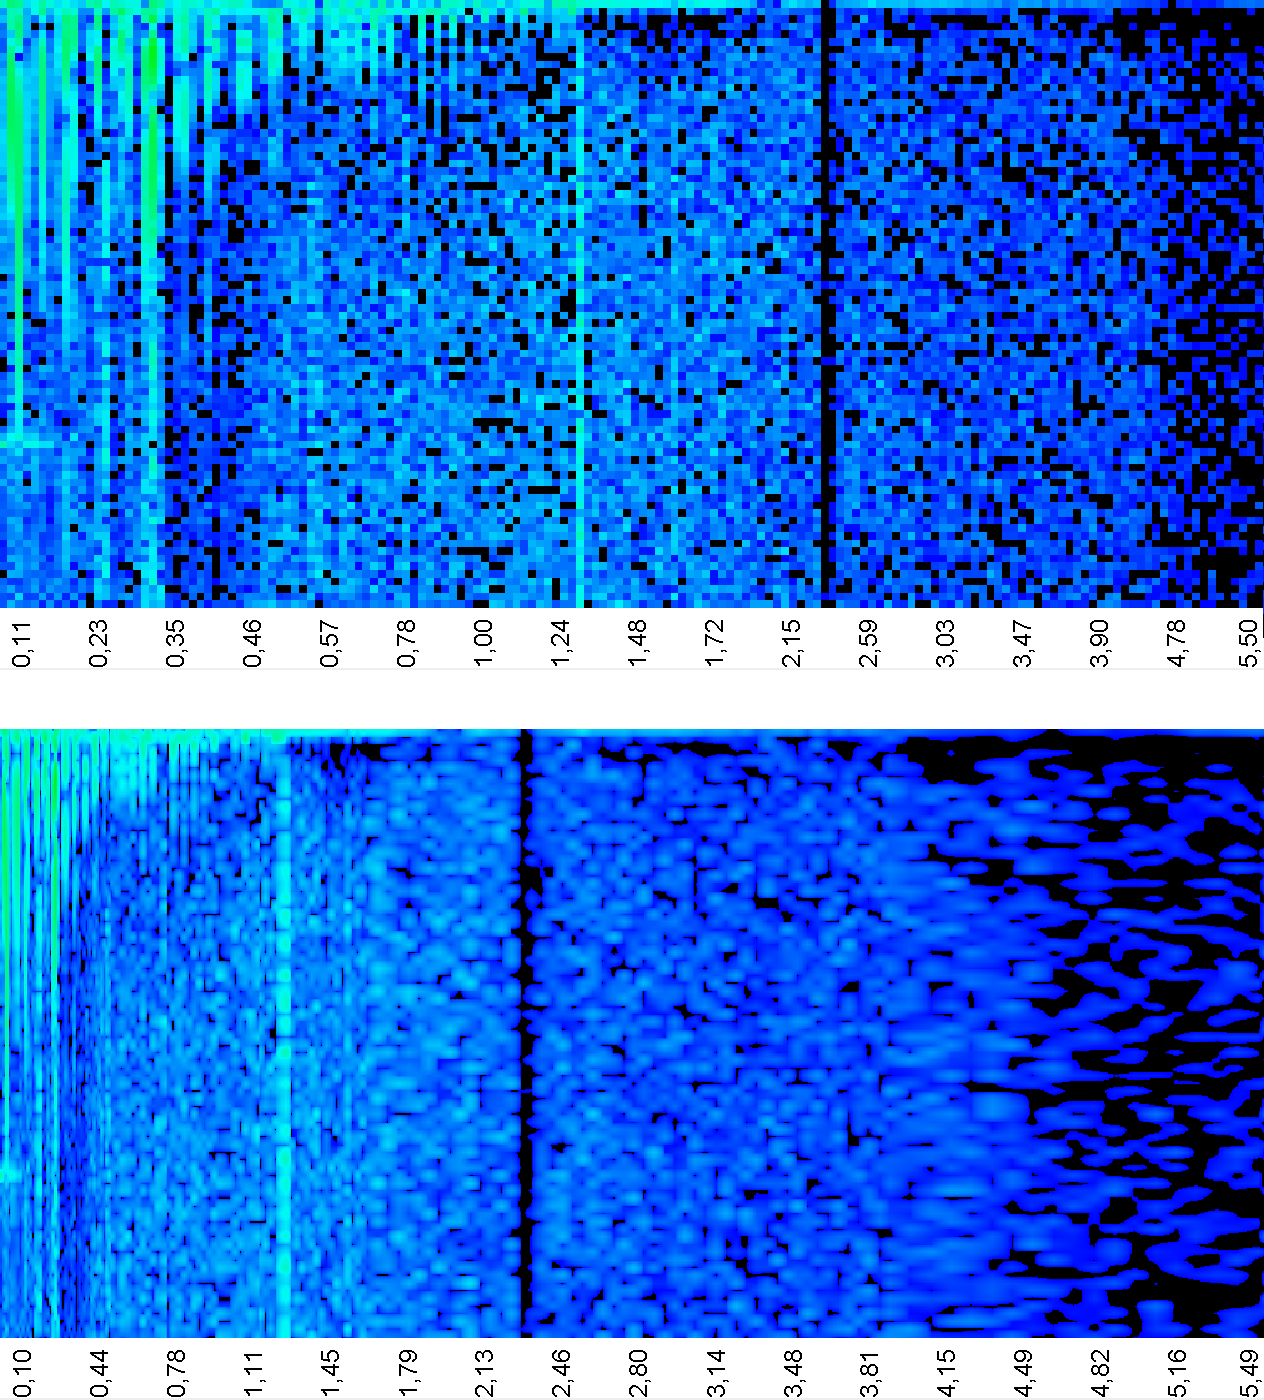
\includegraphics[width=140mm]{images/even_and_uneven_ionogram.png}
	\caption{In the top part of this figure, a ionogram is presented. In the bottom part, an evenly sampled ionogram created from the top one is presented. It is worth notice that the labels of horizontal (frequency) aces of the top ionogram are unevenly distributed. Data from orbit 3874, frame 0 \citep{FTP}.}
	\label{fig:even_uneven_iono}
\end{figure}

\section{Title of the second subchapter of the second chapter}
